% Options for packages loaded elsewhere
% Options for packages loaded elsewhere
\PassOptionsToPackage{unicode}{hyperref}
\PassOptionsToPackage{hyphens}{url}
%
\documentclass[
  number,
  preprint]{elsarticle}
\usepackage{xcolor}
\usepackage{amsmath,amssymb}
\setcounter{secnumdepth}{5}
\usepackage{iftex}
\ifPDFTeX
  \usepackage[T1]{fontenc}
  \usepackage[utf8]{inputenc}
  \usepackage{textcomp} % provide euro and other symbols
\else % if luatex or xetex
  \usepackage{unicode-math} % this also loads fontspec
  \defaultfontfeatures{Scale=MatchLowercase}
  \defaultfontfeatures[\rmfamily]{Ligatures=TeX,Scale=1}
\fi
\usepackage{lmodern}
\ifPDFTeX\else
  % xetex/luatex font selection
\fi
% Use upquote if available, for straight quotes in verbatim environments
\IfFileExists{upquote.sty}{\usepackage{upquote}}{}
\IfFileExists{microtype.sty}{% use microtype if available
  \usepackage[]{microtype}
  \UseMicrotypeSet[protrusion]{basicmath} % disable protrusion for tt fonts
}{}
\makeatletter
\@ifundefined{KOMAClassName}{% if non-KOMA class
  \IfFileExists{parskip.sty}{%
    \usepackage{parskip}
  }{% else
    \setlength{\parindent}{0pt}
    \setlength{\parskip}{6pt plus 2pt minus 1pt}}
}{% if KOMA class
  \KOMAoptions{parskip=half}}
\makeatother
% Make \paragraph and \subparagraph free-standing
\makeatletter
\ifx\paragraph\undefined\else
  \let\oldparagraph\paragraph
  \renewcommand{\paragraph}{
    \@ifstar
      \xxxParagraphStar
      \xxxParagraphNoStar
  }
  \newcommand{\xxxParagraphStar}[1]{\oldparagraph*{#1}\mbox{}}
  \newcommand{\xxxParagraphNoStar}[1]{\oldparagraph{#1}\mbox{}}
\fi
\ifx\subparagraph\undefined\else
  \let\oldsubparagraph\subparagraph
  \renewcommand{\subparagraph}{
    \@ifstar
      \xxxSubParagraphStar
      \xxxSubParagraphNoStar
  }
  \newcommand{\xxxSubParagraphStar}[1]{\oldsubparagraph*{#1}\mbox{}}
  \newcommand{\xxxSubParagraphNoStar}[1]{\oldsubparagraph{#1}\mbox{}}
\fi
\makeatother


\usepackage{longtable,booktabs,array}
\usepackage{calc} % for calculating minipage widths
% Correct order of tables after \paragraph or \subparagraph
\usepackage{etoolbox}
\makeatletter
\patchcmd\longtable{\par}{\if@noskipsec\mbox{}\fi\par}{}{}
\makeatother
% Allow footnotes in longtable head/foot
\IfFileExists{footnotehyper.sty}{\usepackage{footnotehyper}}{\usepackage{footnote}}
\makesavenoteenv{longtable}
\usepackage{graphicx}
\makeatletter
\newsavebox\pandoc@box
\newcommand*\pandocbounded[1]{% scales image to fit in text height/width
  \sbox\pandoc@box{#1}%
  \Gscale@div\@tempa{\textheight}{\dimexpr\ht\pandoc@box+\dp\pandoc@box\relax}%
  \Gscale@div\@tempb{\linewidth}{\wd\pandoc@box}%
  \ifdim\@tempb\p@<\@tempa\p@\let\@tempa\@tempb\fi% select the smaller of both
  \ifdim\@tempa\p@<\p@\scalebox{\@tempa}{\usebox\pandoc@box}%
  \else\usebox{\pandoc@box}%
  \fi%
}
% Set default figure placement to htbp
\def\fps@figure{htbp}
\makeatother





\setlength{\emergencystretch}{3em} % prevent overfull lines

\providecommand{\tightlist}{%
  \setlength{\itemsep}{0pt}\setlength{\parskip}{0pt}}



 
\usepackage[]{natbib}
\bibliographystyle{elsarticle-num}


\makeatletter
\@ifpackageloaded{caption}{}{\usepackage{caption}}
\AtBeginDocument{%
\ifdefined\contentsname
  \renewcommand*\contentsname{Table of contents}
\else
  \newcommand\contentsname{Table of contents}
\fi
\ifdefined\listfigurename
  \renewcommand*\listfigurename{List of Figures}
\else
  \newcommand\listfigurename{List of Figures}
\fi
\ifdefined\listtablename
  \renewcommand*\listtablename{List of Tables}
\else
  \newcommand\listtablename{List of Tables}
\fi
\ifdefined\figurename
  \renewcommand*\figurename{Figure}
\else
  \newcommand\figurename{Figure}
\fi
\ifdefined\tablename
  \renewcommand*\tablename{Table}
\else
  \newcommand\tablename{Table}
\fi
}
\@ifpackageloaded{float}{}{\usepackage{float}}
\floatstyle{ruled}
\@ifundefined{c@chapter}{\newfloat{codelisting}{h}{lop}}{\newfloat{codelisting}{h}{lop}[chapter]}
\floatname{codelisting}{Listing}
\newcommand*\listoflistings{\listof{codelisting}{List of Listings}}
\makeatother
\makeatletter
\makeatother
\makeatletter
\@ifpackageloaded{caption}{}{\usepackage{caption}}
\@ifpackageloaded{subcaption}{}{\usepackage{subcaption}}
\makeatother
\journal{Computers in Biology and Medicine}
\usepackage{bookmark}
\IfFileExists{xurl.sty}{\usepackage{xurl}}{} % add URL line breaks if available
\urlstyle{same}
\hypersetup{
  pdftitle={Increasing the accuracy of ST-segment elevation detection in an ECG through automated visual rules},
  pdfauthor={Lukas Hughes-Noehrer; Gabriel Strain; Adina Rahim; James Sinnott; Jonathan Carlton; Crystal T. Wu; Richard Body; Caroline Jay},
  pdfkeywords={electrocardiogram, ST
elevation, visualisation, crowdsourced, user validation},
  hidelinks,
  pdfcreator={LaTeX via pandoc}}


\setlength{\parindent}{6pt}
\begin{document}

\begin{frontmatter}
\title{Increasing the accuracy of ST-segment elevation detection in an
ECG through automated visual rules}
\author[1]{Lukas Hughes-Noehrer%
\corref{cor1}%
}
 \ead{lukas.noehrer@manchester.ac.uk} 
\author[1]{Gabriel Strain%
%
}

\author[2]{Adina Rahim%
%
}

\author[2]{James Sinnott%
%
}

\author[1]{Jonathan Carlton%
%
}

\author[1]{Crystal T. Wu%
%
}

\author[3]{Richard Body%
%
}

\author[1]{Caroline Jay%
%
}


\affiliation[1]{organization={The University of Manchester, Department
of Computer Science},addressline={Oxford
Road},city={Manchester},country={United
Kingdom},countrysep={,},postcode={M13 9PL},postcodesep={}}
\affiliation[2]{organization={The University of Manchester, Research IT,
IT Services},addressline={Oxford Road},city={Manchester},country={United
Kingdom},countrysep={,},postcode={M13 9PL},postcodesep={}}
\affiliation[3]{organization={The University of Manchester, Division of
Cardiovascular Sciences},addressline={Oxford
Road},city={Manchester},country={United
Kingdom},countrysep={,},postcode={M13 9PL},postcodesep={}}

\cortext[cor1]{Corresponding author}








        
\begin{abstract}
Accurate identification of ST‑segment elevation on the electrocardiogram
(ECG) is essential for diagnosing acute myocardial infarction, yet
interpretation remains challenging due to noise, signal variability,
differences in user expertise and limitations of existing automated
methods. This study investigates whether novel, clinically motivated
visualisation techniques -- including a novel heart‑rate--corrected
ST‑analysis window (STc) -- can make ST‑segment elevation easier to
detect. (Part I) qualitative validation interviews with practising
clinicians from emergency medicine, anaesthesia, critical care and
cardiology, followed by (Part II) a preregistered online experiment with
members of the public unfamiliar with ECG interpretation.

In the clinician interviews (n = 6), participants described the
visualisations as transparent, clinically coherent, helpful for
training, and complementary to automated prompts. Clinicians
particularly valued visual cues that provided a consistent and
physiologically grounded ST‑analysis window; for this reason, we
included STc, a heart‑rate--corrected interval that avoids reliance on
arbitrary fixed millisecond cut-offs and mitigates heart‑rate--driven
distortions in defining the end of the ST‑segment.

Overall, the findings demonstrate that intuitive, explainable visual
cues can support accurate detection of ST‑segment elevation and have
potential for future clinical decision‑support tools, training
resources, and patient‑facing applications. We conducted a mixed‑methods
investigation comprising two components: In the online experiment (n =
303), participants classified single‑lead, single‑beat ECG images that
either incorporated visualisations or displayed the visually unannotated
signal. Accuracy and response times, analysed using generalised linear
mixed models, showed that participants made significantly more accurate
and faster decisions when visualisations were present. Performance
differed across visualisation types: shading‑based designs were most
effective when ST‑segment elevation was present, while J‑point markers
were particularly helpful when elevation was absent.
\end{abstract}





\begin{keyword}
    electrocardiogram \sep ST
elevation \sep visualisation \sep crowdsourced \sep 
    user validation
\end{keyword}
\end{frontmatter}
    

\section{Introduction}\label{introduction}

Cardiovascular diseases remain the leading cause of death worldwide,
accounting for an estimated 19.8 million deaths in 2022. Approximately
85\% of these were due to heart attack and stroke \cite{who}. Myocardial
Infarction (MI), commonly known as a heart attack, is therefore a major
global health concern \cite{moraes_2017, ibanez_2018}. The
electrocardiogram (ECG or EKG) is an important diagnostic tool for the
investigation of heart attacks and heart problems, and is interpreted
using visualisations of the electrical impulses flowing through the
heart. ECGs are quick, cost-effective, and non-invasive, and are
therefore usually the first investigation a patient presenting with a
suspected cardiac issue may undergo \cite{hampton_2024}.

Despite their ubiquity as a medical diagnostic tool, ECGs are
notoriously difficult to interpret
\cite{salerno_2003, cook_2020, rafie_2021}. Accuracy in ECG
interpretation varies, even amongst those trained in cardiology. A 2020
meta-analysis of 78 studies across all levels of clinical training
reported a median accuracy rate of 54\% \cite{cook_2020}. Expectedly, as
medical professionals move through their careers, undergo additional
training, and gain further experience, accuracy trends upwards. Yet,
resident doctors (those still in training) make up significant
proportions of medical workforces \cite{nhs_stats}, and errors in ECG
interpretation account for poor patient health outcomes and preventable
deaths \cite{mele_2008}. Improving ECG interpretation remains a critical
issue.

Historically, computer-assisted interpretation of ECGs dates back to the
1950s \cite{macfarlane_automated_2021}, and algorithmic support is now
standard in ECG monitoring systems. Contemporary Computerised
Interpretation of ECG (CIE) aims to reduce diagnostic errors and support
clinical decision-making, yet studies have demonstrated the fallibility
of automated interpretations; clinician oversight is required to avoid
misdiagnosis
\cite{smulyan_computerized_2019, schlapfer_computer-interpreted_2017}.
Recent advances in Artificial Intelligence (AI) and Machine Learning
(ML), coupled with large waveform datasets, have enabled methods ranging
from rule-based systems to deep learning approaches
\cite{gupta_computer-interpreted_2024, gill_artificial_2023, lyon_computational_2018}.
Despite promising clinical trials and regulatory approval of some
devices \cite{himmelreich_diagnostic_2023}, adoption remains limited due
to systemic bias, liability concerns, cybersecurity risks, and
unresolved technical and ethical challenges
\cite{khurshid_clinical_2023, siontis_artificial_2021, elul_meeting_2021, chung_clinical_2022, rajpurkar_ai_2022}.
Trust in AI systems remains a critical barrier, with clinicians
expressing cautious optimism, but highlighting issues around cost,
usability, and explainability
\cite{schepart_artificial_2023, stewart_attitudes_2024, burgess_healthcare_2023, asan_artificial_2020}.
Automated techniques that can reliably support the intuitive
understanding of ECG data are therefore particularly important.

The majority of work examining ECG interpretation has taken place with
medical practitioners. While various studies have investigated how
practitioners with different levels of ECG-interpretation experience
read ECGs \cite{cook_2020, davies_2019, attar_2025}, to our knowledge,
Alahmadi et al.~\cite{alahmadi_2019a, alahmadi_2019b, alahmadi_2020} is
the only work focused on the interpretation of ECGs (detecting prolonged
QT intervals) by lay people. Building on this, along with our recent
work demonstrating that explainable visualisation techniques are useful
for facilitating the interpretation of ECGs and aiding clinical
decision-making \cite{hughes_2025, noehrer}, we developed novel
ST-segment elevation (ST-elevation) visualisations informed by
established clinical rules routinely used by medical professionals
\cite{rao_2025}. Our visualisations highlight areas that are of interest
to clinicians, with the aim of supporting efficient, accurate ECG
interpretation. To assess the effectiveness of our visualisations, we
adopted a mixed-methods approach: a clinical user validation --
presented in Part I -- and a reproducible single-experiment study with
lay participants -- presented in Part II. We selected lay people to
evaluate the usefulness of our visualisation under the assumption that
if individuals with no prior experience in interpreting ECGs can
accurately identify ST-elevation, it provides strong evidence for the
comprehensibility and the intuitiveness of our explainable designs.

\subsection{Hypotheses}\label{hypotheses}

Our Part II study tested three visualisations based on clinical rules
with the aim of scaffolding understanding and interpretation of
ST-elevations. Owing to the novelty of both the designs and the testing
of lay populations with ECG visualisations, we do not hypothesise that
one design may be superior to another. Previous evidence that novel
designs can be beneficial with regards to the interpretation of ECG data
among lay
participants\textasciitilde{}\citep{alahmadi_2019a, alahmadi_2019b, alahmadi_2020, alahmadi_2021, alahmadi_2023}
lead to the following hypotheses, both of which were pre-registered with
the Open Science Framework\footnote{\url{https://osf.io/v6tjp}}:

\begin{itemize}
\item
  H1: Participants' performance on a binary decision task recognising the presence or absence of ST-elevation will be more accurate when a visualisation condition is present as opposed to when there is no additional visualisation beyond what is standard for ECG data.
\item
  H2: Participants will make binary classification decisions significantly more quickly when additional visualisations are present compared to when they are not.
\end{itemize}

\section{Related Work}\label{related-work}

Myocardial Infarction (MI) refers to a partial or complete blockage of
the blood flow to a portion of the heart
muscle\textasciitilde{}\citep{ojha_2023}. Such a blockage deprives parts
of the heart of oxygen, potentially leading to cell death and necrosis.
Depending on the extent of this oxygen deprivation, MI can range from
being symptomless (undetected by the affected person), to catastrophic,
leading to sudden death. Types of MI are diagnosed based on the presence
of cardiac bio-markers in the blood concurrent with other criteria,
including changes in the electrical activity of the
heart\textasciitilde{}\citep{thygesen_2019} detected using an ECG. In a
clinical setting, 10 electrodes are attached to different parts of the
patient's body to produce 12 different ``views'\,' of the heart's
electrical activity\textasciitilde{}\citep{hampton_2024}; these are
often referred to as \emph{leads}. ST-segment elevation Myocardial
Infarction (STEMI) is diagnostically defined
as\textasciitilde{}\citep{rao_2025, akbar_2024}:

\begin{quotation}
  The presence of an ST-segment that is elevated above the baseline at the 
  J-point by at least 0.1~millivolts (mV) in any two contiguous leads except V2 and V3.
  In leads V2 and V3, this elevation must be at least 0.2~mV in males aged 40 years or older,
  at least 0.25~mV in males aged under 40 years, and at least 0.15~mV in females.
\end{quotation}

\subsection{ST-Elevation Myocardial
Infarction}\label{st-elevation-myocardial-infarction}

\begin{figure}

\centering{

\pandocbounded{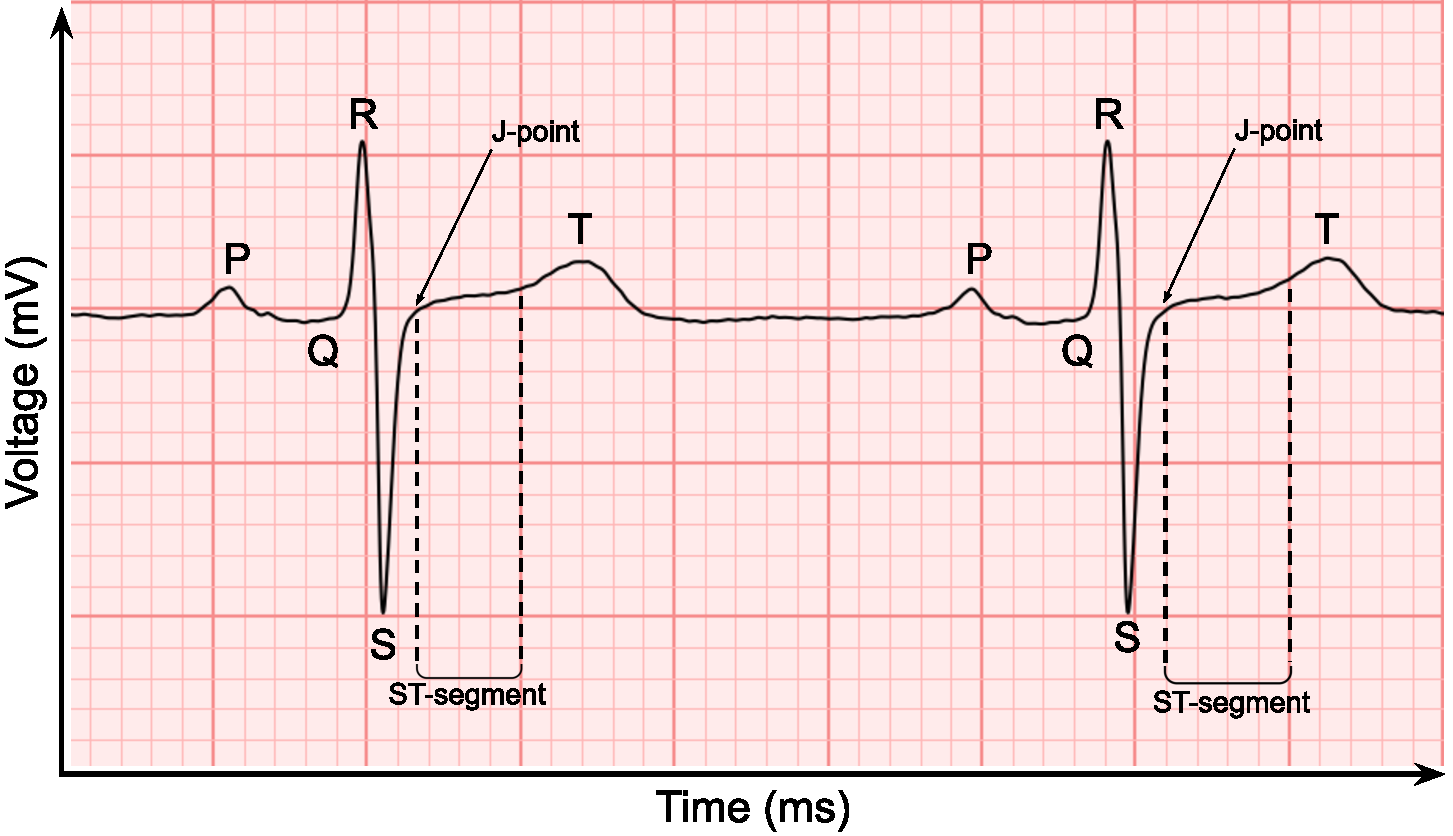
\includegraphics[keepaspectratio]{graphics/ecg-example.pdf}}

}

\caption{\label{fig-ecg-signal-explainer}Phases of the ECG: Using real
ECG data from the V4 chest lead to illustrate the P-wave, the QRS
complex, the ST-segment,the T-wave, and the J-point. In the experiment,
participants were instructed to classify ECG signals such as these as
\texttt{ST-elevation\textquotesingle{}\ or}No ST-elevation'. This
particular signal does not show ST-elevation. Each small red square
represents 40\textasciitilde milliseconds (ms) horizontally and
0.1\textasciitilde millivolts (mV) vertically. Each large red square
represents 200\textasciitilde milliseconds horizontally and
0.5\textasciitilde millivolts vertically.}

\end{figure}%

In this context, \emph{contiguous} refers to leads that represent
adjacent anatomical areas.
Figure\textasciitilde{}\ref{fig-ecg-signal-explainer} illustrates the
different parts of a typical ECG signal, including the P-wave, QRS
complex, ST-segment, J-point, and T-wave. In the context of ECG
investigations, heart attacks featuring ST-segment elevation (STEMI) are
differentiated from those where this elevation is absent (NSTEMI); the
former is more severe, and so is studied in this work. Survival
following a STEMI has improved substantially over the past few
decades\textasciitilde{}\citep{pascual_2020, pedersen_2014, gale_2014}.
Despite this, STEMI and other forms of MI remain a leading cause of
mortality\textasciitilde{}\citep{moraes_2017, ibanez_2018} and lower
Health-Related Quality of Life
(HRQoL)\textasciitilde{}\citep{wang_2014, kang_2016, bahall_2018}
worldwide. Generally, prompt diagnosis and treatment are crucial for
reducing mortality, limiting the duration of a person's hospital stay,
and for their prognosis following a STEMI
event\textasciitilde{}\citep{ibanez_2018}. Any intervention that may
improve clinicians' (and potentially patients') ability to quickly
recognise STEMI is therefore worthy of study.

\subsection{ECG Interpretation}\label{ecg-interpretation}

ECG interpretation is a complex problem, even for clinicians with years
of training\textasciitilde{}\citep{salerno_2003, cook_2020, rafie_2021}.
In a clinical context, the heart activity taken from all 12 ECG leads is
interpreted. Even recordings as short as 10\textasciitilde seconds (s)
of heart activity information become complex data when taking into
account 12 different signals, and clinicians are taught to make
diagnoses based on the ensemble of information
available\textasciitilde{}\citep{hampton_2024}. Nevertheless,
single-lead views offer substantial amounts of information, and require
far less time and training to be able to interpret; we focus on
single-lead, single-heartbeat ECG data for the presented experiment with
lay participants.

When using ECG to help diagnose STEMI, the criteria are relatively
simple; elevation in two contiguous leads at a certain point in the
signal. Of course, this requires a huge amount of processing when
examining a full 12-lead ECG, as elevation can occur in any single
heartbeat over 12 different leads, and clinicians often work under
substantial time pressure. \%In addition to the amount of data that must
be considered, actual ECGs are often noisy to the point of ambiguity.
Over several studies, clinicians were reported as having an overall
accuracy rating of around
70\%\textasciitilde{}\citep{mccabe_2013, veronese_2016} and low levels
of interrater agreement, with a kappa value of 0.33 reported in McCabe
et al.\textasciitilde{}\citep{mccabe_2013}. Studies have indicated that
these issues may be due to difficulties in correctly identifying the
J-point\textasciitilde{}\citep{carley_2002} or confusion that arises
when the level of ST-elevation is very
low\textasciitilde{}\citep{erling_2004}. While increased training
improves accuracy on ECG interpretation
paradigms\textasciitilde{}\citep{mccabe_2013, veronese_2016, cook_2020},
the fact remains that interpreting ECG is difficult, even for those
whose speciality is cardiology and those with many years of training and
experience.

\subsection{ECG Visualisation}\label{ecg-visualisation}

The way in which ECG data are presented to clinicians has changed little
since the invention of the technique over a century
ago\textasciitilde{}\citep{friedman_2024}; the quintessential form of
the ECG, and the issues that clinicians face when engaging with it,
remain much the same. ECGs are typically drawn on a Cartesian line graph
with the signal voltage in millivolts on the (y)-axis and time in
milliseconds (ms) on the (x)-axis. A background grid system is employed
to aid interpretation;
Figure\textasciitilde{}\ref{fig-ecg-signal-explainer} illustrates this
system. Whether produced manually by a pen on grid paper, or drawn
digitally by a computer, the resulting visualisation is essentially
identical. Clinicians are expected to analyse the ensemble of ECG data
together, and are not typically assisted by any visual aids, such as
labels or markings, other than those that name the leads themselves and,
if supported, computer-automated interpretations printed as text.

Chest and limb leads have been combined separately into a pair of
3-dimensional views of the heart's electrical activity by Chiang et
al.\textasciitilde{}\citep{chiang_2001} and Heo et
al.\textasciitilde{}\citep{heo_2020}; this technique has received some
approval from clinicians based on
polling\textasciitilde{}\citep{chiang_2001}, and has been used
successfully in algorithmic classification
paradigms\textasciitilde{}\citep{heo_2020, fang_2022, bortolan_2023}.
Kors and van Herpern\textasciitilde{}\citep{kors_2008} and Wagner et
al.\textasciitilde{}\citep{wagner_2008} have explored the theoretical
use of ``inverted'\,' (mirror image) ECG leads, finding mixed results
with regards to their benefit over traditional, 12-lead ECG. Perron et
al.\textasciitilde{}\citep{perron_2006}, however, found that including 7
additional inverted leads provided benefits in terms of detecting
artificially induced arterial blockage. Other visualisation techniques
have included glyph-based interactive
systems\textasciitilde{}\citep{xu_2018}, vectorial methods to illustrate
the magnitude and direction of the electrical impulses of the
heart\textasciitilde{}\citep{burch_1953, burch_1985, riera_2007, jaros_2019},
and spatial techniques that generate maps of electrical potentials
across the body (Body Surface Potential Mapping or
BSPM)\textasciitilde{}\citep{lux_1978, taccardi_1998}. These
visualisation techniques, while sometimes useful for clinicians, are
only ever considered as supplementary to traditional ECG
visualisations\textasciitilde{}\citep{bond_2013}; their advantage is
that they increase the amount and/or the complexity of the data
displayed, meaning such techniques would not be suitable for those with
no experience interpreting ECGs. The visualisation techniques presented
in this work are designed to increase the salience of relevant
visualisation features, as opposed to simply adding information.

\subsection{Using Clinical Rules to Guide Visualisation
Design}\label{using-clinical-rules-to-guide-visualisation-design}

Clinical decision rules and protocols can be used to guide the design of
healthcare data visualisations by translating clinical knowledge into
structured representations. Such rules commonly take the form of
thresholds, scoring systems, or rule-based pathways that support
recognition of abnormal states, escalation of care, and coordination of
clinical response; subsequently informing clinical
decisions\textasciitilde{}\cite{sutton_overview_2020}. In medical
informatics, there is growing recognition of the need for effective data
visualisations to overcome information overload and enable users to
recognise clinically meaningful changes more effectively than when using
raw data alone\textasciitilde{}\citep{aigner_2008}. Similarly, visual
aggregation and structured timelines can promote more consistent
interpretation of complex health
data\textasciitilde{}\cite{ledesma_health_2019} and enhance situational
awareness (SA) in clinical practice\textasciitilde{}\citep{dixit_2020}.

However, the effectiveness of such visualisations is closely tied to how
information is visually encoded and subsequently interpreted. Visual
design choices directly shape perceptual processing and reasoning,
meaning that poor encoding can undermine decision-making even when
underlying data or logic are sound\textasciitilde{}\cite{ware2012}.
Design studies in applied visualisation further emphasise that
mismatches between visual representations, user tasks, and context of
use frequently lead to limited adoption or
misuse\textasciitilde{}\cite{sedlmair_design_2012}.

Visualisations are also increasingly used to inform lay audiences about
their health data and facilitate their understanding of complex
information\textasciitilde{}\citep{arcia_2024}. In these settings,
decision rules and algorithmic assessments are often embedded within
visual summaries, indicators, or feedback messages, shaping how users
perceive their health status and the actions they choose to take. This
further reinforces the importance of aligning visualisation design with
the needs, expectations, and capabilities of specific audiences.

Clearly defined communication goals, the guiding of design through
taxonomies, and evaluation based on audience-specific outcomes are
essential for the successful design of visualisations for any
audience\textasciitilde{}\citep{ancker_2024}. These principles emphasise
that the success of clinical decision rules and protocols cannot be
assessed independently of their visual representation, and that
effective visualisation plays a central role in determining whether such
systems support understanding, trust, and appropriate action.

\subsection{Future Forward: Wearable Health
Technologies}\label{future-forward-wearable-health-technologies}

A further driver for novel visualisations and the need for health data
to be easily understood is the rapid adoption of wearable health
technologies\textasciitilde{}\citep{ma_making_2025, hicks_best_2019}.
The recently released NHS 10 Year Health Plan highlights a move away
from hospital to community care, a shift from analogue to digital, and
an emphasis on prevention over
treatment\textasciitilde{}\citep{dhsc_2025}. The provision of wearable
health monitors, such as smartwatches, fitness bands, and intelligent
jewellery, is seen as central to the delivery of this ambitious plan.
Most of these devices now include ECG capabilities and allow their
wearers to record single, and sometimes multi-lead, ECGs. Some devices
now incorporate complex algorithms capable of warning users if their
vital signs deviate from normal thresholds. Whilst mostly focused on the
detection of arrhythmias (e.g., Atrial
Fibrillation\textasciitilde{}\citep{abdelrazik_2025}), there is ongoing
exploration of their role in acute coronary
syndromes\textasciitilde{}\citep{choi_2025, neri_2023}. Wearables are
able to support patient care wherever the patient happens to be
situated, facilitating diagnostics beyond the hospital and enabling a
more comprehensive view of a patient's health. They can further empower
their users to take on a more active role in their healthcare by
providing data and personalised feedback, and encouraging
self-monitoring, adherence to healthy lifestyles, and informed dialogues
with care providers\textasciitilde{}\citep{ehizogie_2024}. Wearables,
and digital technology more generally, can also contribute to the health
literacy of young people and their understanding about their own
health\textasciitilde{}\citep{goodyear_2019}. While live monitoring of
ECG data from consumer-grade wearable devices is not yet a reality, its
inevitability, combined with the wider benefits conferred by constant
monitoring and the democratisation of healthcare, indicate the benefits
of studying ECG visualisation with lay people as well as clinical
experts.

\section{Materials and Methodology}\label{materials-and-methodology}

This section outlines our overall research methodology, encompassing the
algorithm development and visualisation design, the collection of
clinician feedback on the proposed visualisations, and the lay‑person
experiment.

\subsection{Algorithm Development}\label{algorithm-development}

The codebase of our full
pipeline\footnote{\url{https://github.com/ECG-X/ECG-X_ST-segment-feature-detection-and-visualisation}}
is openly available on GitHub under a dual-licensing model: released for
non-commercial use under the Creative Commons
Attribution‑NonCommercial‑ShareAlike 4.0 International Licence (CC
BY‑NC‑SA 4.0), with alternative commercial licensing available upon
request. We describe the assumptions made and discuss our algorithm in
detail, from data preparation and preprocessing to how we detect crucial
ECG features for ST-segment analysis. This includes a newly introduced
method to correct the duration of an ST-segment and the reasons behind
our visualisation design.

\subsubsection{Technical Assumptions}\label{technical-assumptions}

As our algorithm was intentionally designed to produce novel,
foundational, human-understandable visualisations to facilitate the
interpretation of ECGs, the following assumptions were made:

\begin{itemize}
    \item Given the complexity and variety of raw ECG signals, we acknowledge that our pipeline is tuned to suit the PTB Diagnostics database~\cite{ptb} specifically, containing clinically labelled, high-quality signals.
    \item We focus on the human-algorithm interaction aspect of algorithm development, using well-known, standard open-source processing packages and algorithms for ECG signal processing.
    \item The proposed visualisation pipeline prioritises perceptual clarity and interpretability over optimal representation of physiological states. Our contribution lies in novel \textit{clinical rule-based visualisations} intended to standardise visual representation rather than to model underlying electrophysiology with maximal accuracy. This design choice reflects the development focus on human interpretation and decision support rather than physiological measurement accuracy (a common trade‑off in CIE design rather than a limitation specific to our method).
\end{itemize}

\subsubsection{Data Preparation}\label{data-preparation}

Raw ECG data were acquired from the clinically-validated PTB Diagnostic
ECG Database\textasciitilde{}\cite{ptb}, which is openly available and
can be downloaded from PhysioNet. Prior to any signal processing, the
raw data were converted from WaveForm DataBase (WFDB) format to CSV for
ingestion into our
\textit{ST-segment feature detection and visualisation} pipeline. From
the 549 available datasets downloaded and converted to CSV, we grouped
them into three categories based on the diagnosis (i.e.~reason for
admission) provided by the database. There were 80\textasciitilde ECG
recordings classified as \textit{healthy control}, 368
\textit{myocardial infarction}, and the \textit{other} remaining 101
includes other heart conditions (e.g., cardiomyopathy, bundle branch
block, etc.) and miscellaneous. We selected data from the
\textit{healthy control} and the \textit{myocardial infarction} group as
input, as they most likely contain signals without and with
ST-elevation, respectively. Each recording is represented by a CSV file
containing data, including all of the leads provided by the database,
from the same recording session. An ST-segment lasts approximately
80\textasciitilde ms to 120\textsubscript{ms}\cite{sattar2023}, and
since the ECG datasets have varying durations, we configured our
pipeline to sample the first 30\textasciitilde s from each recorded
signal. Each signal therefore has approximately 39 potential ST-segments
(based on the mean real-world heart rate of 79.1 beats per minute
(bpm)\textasciitilde{}\cite{Avram2019}) available for analysis and can
be visually annotated with our visualisations.

\subsubsection{Data Preprocessing}\label{data-preprocessing}

A flowchart depicting our full pipeline is shown in
Figure\textasciitilde{}\ref{fig:vis-pipeline}. We utilised
SciPy\textasciitilde{}\cite{2020SciPy-NMeth} and
NeuroKit2\textasciitilde{}\cite{Makowski2021neurokit}, two openly
available Python libraries, for signal preprocessing tasks. The first
two steps of preprocessing aimed to reduce noise while preserving the
signal morphology.

\begin{figure}[H]

{\centering \pandocbounded{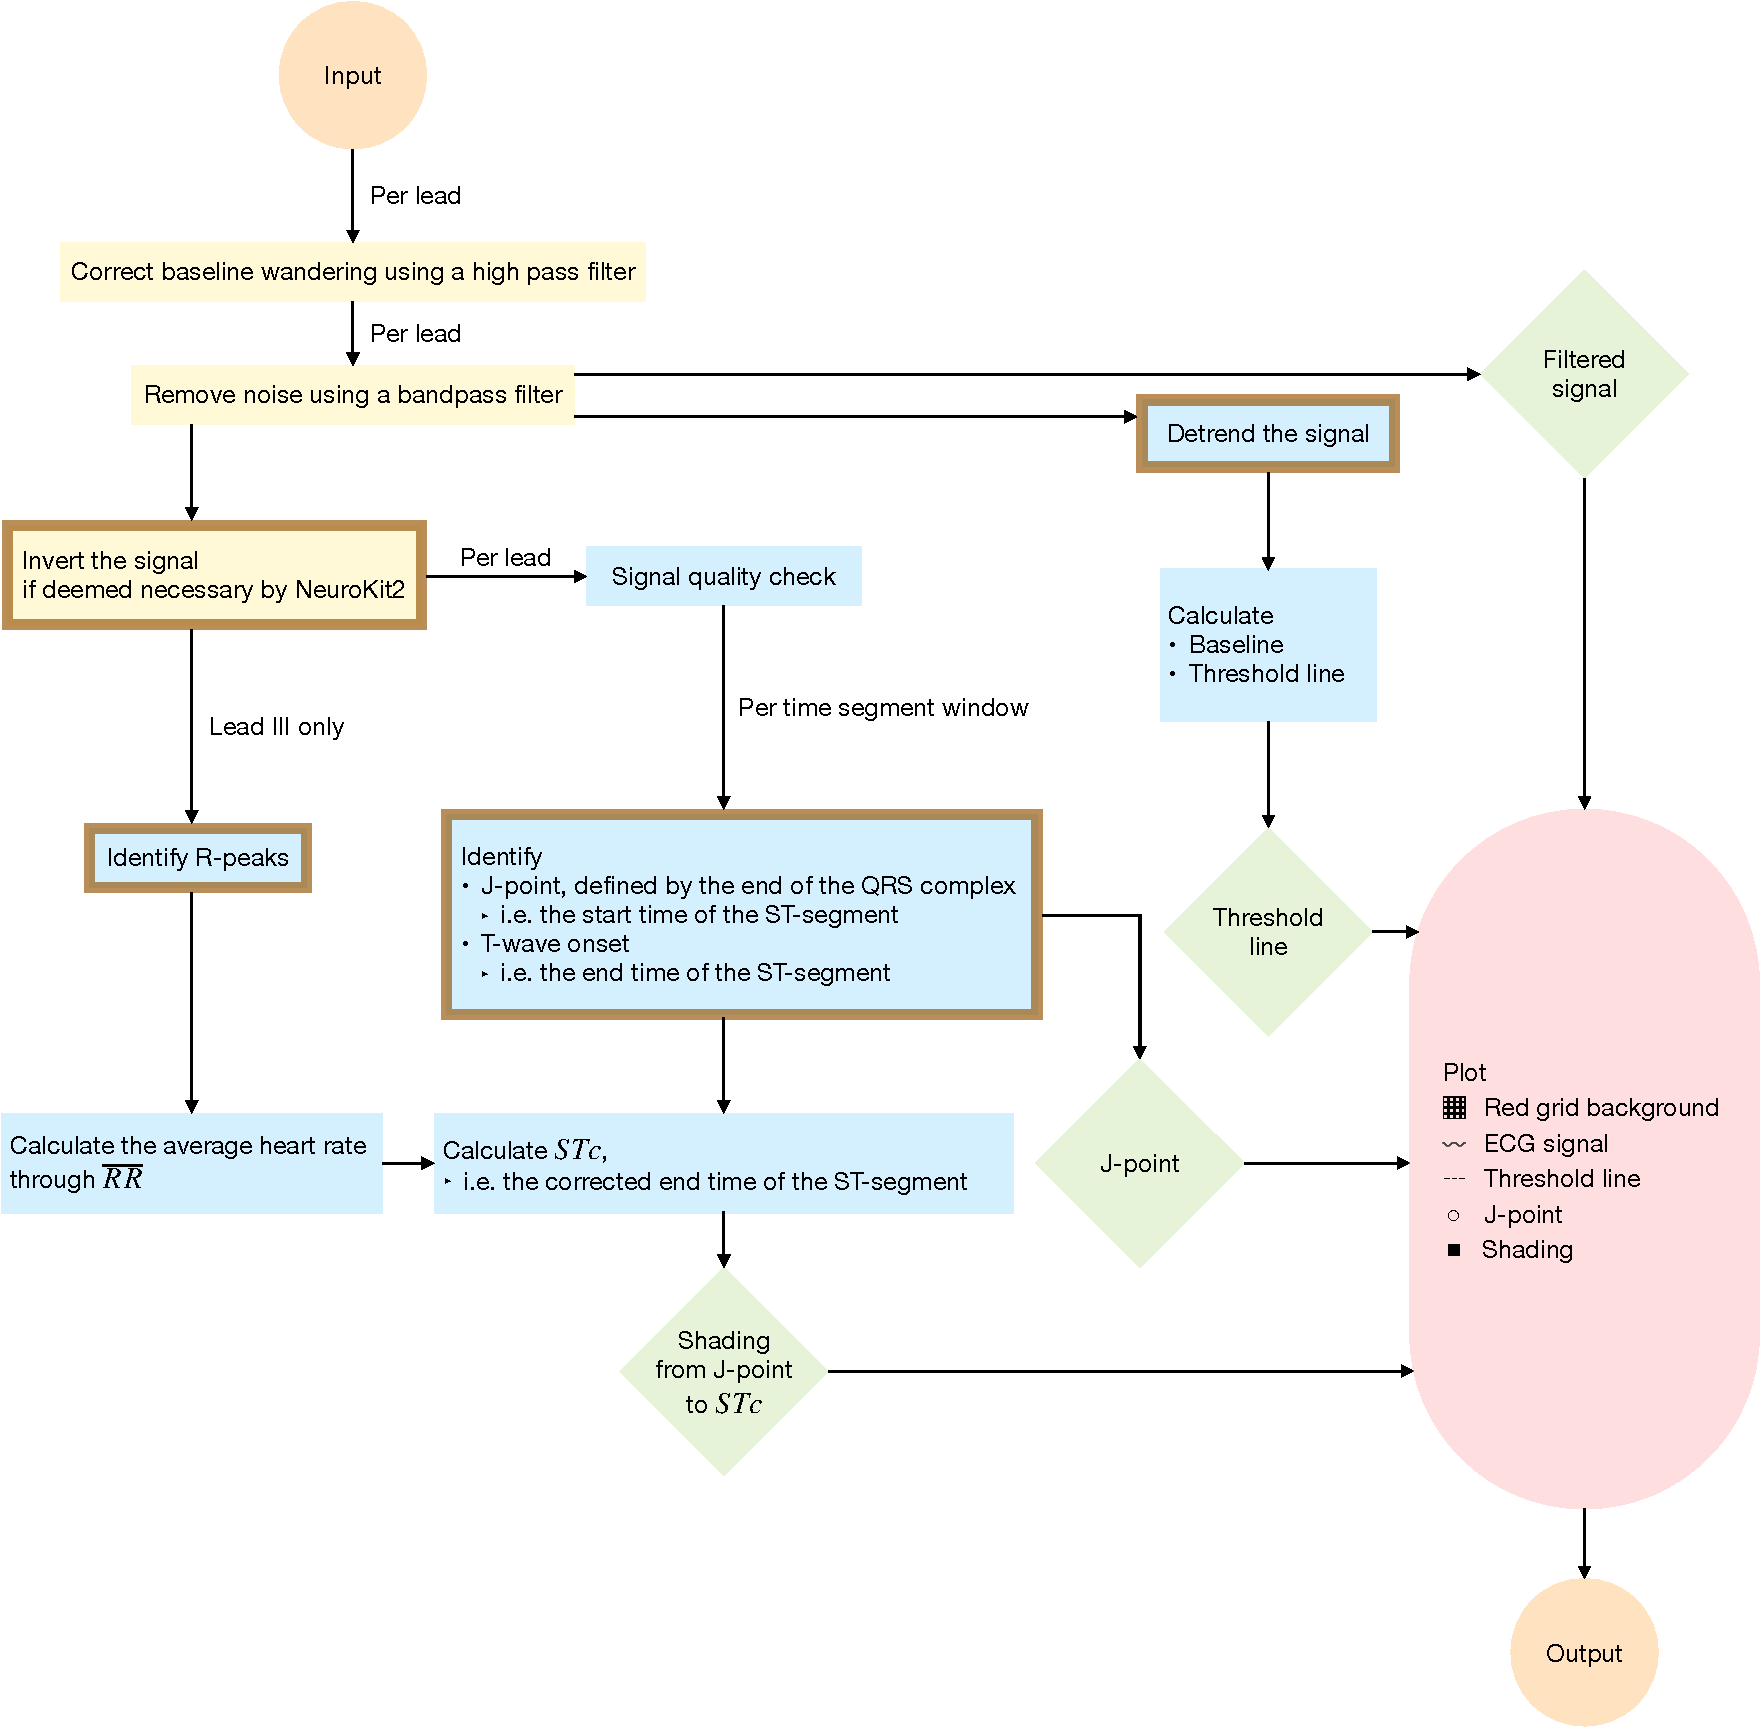
\includegraphics[keepaspectratio]{graphics/vis_pipeline.pdf}}

}

\caption{Computational pipeline for ST-segment features detection and
visualisation: Data preprocessing (in yellow) includes applying a high
pass and a bandpass filter. Some processing is carried out in segments,
each with a duration of the segment time window defined in
configuration. Steps completed utilising NeuroKit2 functions (circled in
brown), identify features relevant to ST-elevations (in blue). The four
distinctive visualisations (in green) are plotted on a red grid
background with the ECG signal (in pink).}

\end{figure}%

Artefacts caused by respiration, movement, electrode impedance, and
electrical interference\textasciitilde{}\cite{Luo2013} distort ECG
signal quality\textasciitilde{}\cite{Zhang2025} and hinder feature
detection relevant to ST-segment interpretation and
analysis\textasciitilde{}\cite{Lenis2017}. To correct baseline wander,
we applied a Butterworth\textasciitilde{}\cite{butterworth1930} high
pass filter, chosen for its accuracy and computational efficiency in
medical applications\textasciitilde{}\cite{Lenis2017}. A cut-off
frequency at 0.5 Hertz
(Hz)\textasciitilde{}\cite{Zhang2025, Kher2019, Kligfield2007} removed
low frequency noise and shifted the signal vertically to centre around
zero. Then, a second Butterworth bandpass filter (0.5\textasciitilde Hz
to 50\textasciitilde Hz) was used to reduce high frequency noise due to
electrical (e.g., powerline) and myoelectric
interferences\textasciitilde{}\cite{Zhang2025, Kher2019, Chatterjee2020},
improving signal clarity. Deflections from the raw signals are preserved
in the filtered signals, which form the basis of the ECG tracings (with
and without visualisations) used in the online experiment with lay
participants.

Our third step utilised NeuroKit2 to identify and invert any
\textit{inverted signals} (an artefact due to electrode placement during
the recording session or pathological
causes\textasciitilde{}\cite{Rosen2014, Rosen2014a, Glancy2014}).
Signals identified to have predominantly upright features with positive
deflection were kept unchanged. This is to support detecting ECG
waveform features, specifically those relevant to an ST-segment.

\subsubsection{Pipeline Configuration and Data Quality
Check}\label{pipeline-configuration-and-data-quality-check}

The pipeline is built to support the 12 conventional leads routinely
used in clinical practice\textasciitilde{}\cite{ashley2004}, where the
leads are selectable through configuration for processing. The algorithm
is also capable of applying the threshold line based on the ST-elevation
criteria depending on the age and sex of the patient. As our online
experiment with lay participants excluded evaluating leads V2 and V3
(see Section\textasciitilde{}\ref{sec-method-online-exp}), the pipeline
was configured accordingly.

ECG signals from the PTB Diagnostic ECG database were measured within
the range of \(\pm 16.384\)\textsubscript{mV}\cite{ptb}, yet ECG
amplitudes are generally below 5\textsubscript{mV}\cite{Xie2020}. For
quality control and to ensure the output ECG images have a consistent
height regardless of signal amplitude, we adopted a conservative
approach by configuring the pipeline to discard datasets with maximum
amplitudes outside \(\pm 3\)\textasciitilde mV, as well as signals
shorter than 30\textasciitilde s. Excluding leads V2 and V3, we
determined 72.5\% (58 out of 80 recordings) and 64.1\% (236 out of 368
recordings) of the datasets from the \textit{healthy control} and the
\textit{myocardial} group, respectively, have maximum amplitudes within
\$\pm\$3\textasciitilde mV. In addition, to streamline the remaining
steps, we partitioned the 30\textasciitilde s signal by a configurable
time segment window (e.g., 5\textasciitilde s) to process. For the final
output, the number of ECG images produced per signal for a lead is
dependent on the specified time segment window and the total duration of
a signal sampled for input.

\subsubsection{Feature Detection}\label{feature-detection}

Recognising ST-elevation requires analysing the signal against the
clinically defined threshold level, an electrical potential displacement
from the signal baseline, and can be computed once the baseline is
established. The baseline, also known as the isoelectric line,
represents net zero electrical
potential\textasciitilde{}\cite{Strauss2021}. As our filtered signal
already centre vertically around zero, we utilised NeuroKit2 to remove
the linear trend and define the resulting signal's mean as our baseline.
Although it approximates the isoelectric line, we acknowledge that our
custom baseline may be skewed towards the side with greater cumulative
deflection in the waveform.

An ST-segment, shown in
Figure\textasciitilde{}\ref{fig-ecg-signal-explainer}, is defined by the
interval from the end of a QRS complex to the start of the following
T-wave. It is typically an isoelectric period near the baseline or may
slope slightly upward in a normal
state\textasciitilde{}\citep{ashley2004, Strauss2021}. We utilised
NeuroKit2 to identify prominent features of each signal, prepared by the
steps discussed in Section\textasciitilde{}\ref{sec-data-preprocess}.
Implementation via NeuroKit2 includes the Martinez et
al.~method\textasciitilde{}\cite{martinez2004} to identify R-peaks and
the discrete wavelet transform (DWT) method to identify onsets and
offsets of relevant waves, including the QRS complex and the T-wave, to
determine an ST-segment and its J-point.

R-peaks are typically the most prominent feature in an ECG tracing and
can be used to compute the average heart rate. We achieved this by
taking the mean of the interval between two consecutive R-peaks
(\(\overline{RR}\)) using data from lead III.

\subsubsection{Novel Correction of ST-segment
Calculations}\label{novel-correction-of-st-segment-calculations}

As previously highlighted, accurately defining the J-point can be
clinically challenging\textasciitilde{}\cite{carley_2002}, and there is
long-standing disagreement and varying practice in defining the
ST-segment and the diagnostic window based on it to detect ST-segment
elevation\textasciitilde{}\cite{man_2017}. A fixed time cut-off, such as
40\textasciitilde ms, 60\textasciitilde ms, or 80\textasciitilde ms
after the J-point, have been widely used, yet their physiological
validity is contested and diagnostic performance is highly sensitive to
chosen offsets\textasciitilde{}\cite{lindow_2020}. As ventricular
repolarisation shortens at high heart rates and lengthens at low heart
rates through rate-dependent action potential adaptation, a fixed delay
from the J-point does not consistently capture the same repolarisation
phase across recordings. As a result, a fixed cut-off to define the
diagnostically-important part of the ST-segment may introduce
heart-rate--dependent distortions in both visual and algorithmic
analysis.

Given these limitations and driven by the need to define a diagnostic
window of the ST-segment for one of our visualisation types introduced
in Section\textasciitilde{}\ref{sec-design-vis}, we developed a novel
algorithm to calculate the ST-segment, \(STc\) (ST corrected), inspired
by Bazett's formula to correct calculation of the QT
interval\textasciitilde{}\citep{bazett}, which is calculated as: \%
\begin{equation*}
STc = \frac{ST}{\sqrt{\overline{RR}}},
\end{equation*} \% where \(STc\) is in milliseconds, \(ST\) is the
duration between the detected J-point and the T-wave onset (ST-segment)
in milliseconds, and the average R-peak to R-peak interval
\(\overline{RR}\) in seconds.

Although \(STc\) uses a Bazett‑type correction where
60\textasciitilde bpm serves as the mathematical reference point
(\(RR = 1\)\textasciitilde s), the algorithm does not assume that all
patients should physiologically behave as if they were at
60\textasciitilde bpm. Rather, 60\textasciitilde bpm is simply the
calibration point that removes the heart‑rate--dependent distortion.
\(STc\) therefore creates a heart‑rate--normalised window that aligns
with the same repolarisation phase at any heart rate, without altering
the ECG signal or imposing a specific physiological state. The resulting
\(STc\) provides a cycle-length--normalised, physiologically coherent
window that is comparable across beats, patients, and varying heart
rates. Unlike fixed cut-offs, which risk sampling different
electrophysiological phases depending on heart rates, \(STc\) ensures
that the analysis window stays consistent. In practice, \(STc\) defines
the duration of the ST-segment, determining its endpoint relative to the
J-point. The resulting heart-rate--normalised diagnostic window is
overlaid in the time domain as a visualisation on the filtered signal,
whose temporal structure remains heart-rate--dependent.

By combining morphology‑based delineation with heart‑rate correction,
\(STc\) provides a robust alternative to conventional post--J‑point
offsets and may yield a more reliable and interpretable framework for
visualising and analysing ST‑segment behaviour in both clinical and
computational applications.

\subsubsection{Visualisations Design and
Algorithm}\label{visualisations-design-and-algorithm}

Based on the features detected by the pipeline, visualisations were
applied (i.e.~visually annotated) on top of the filtered ECG signal. The
visualisations were designed to increase the salience of the visual
features relevant to ST-segment elevation analysis and the subtasks
outlined in Section\textasciitilde{}\ref{sec-method-online-exp}. An
example of each type of visualisation is shown in
Figure\textasciitilde{}\ref{fig:vis-examples}. To reduce the cognitive
load of ECG interpretation tasks, we applied strategies taken from
Cognitive Load Theory (CLT)\textasciitilde{}\citep{paas_2020}. After
iterative cycles of discussion regarding visualising clinical rules for
ST-elevation during the Responsible Research and Innovation (RRI)
workshops, we decided upon a final set of three visualisation types
presented in this study.

All three visualisation types feature a dashed threshold line at
0.1\textasciitilde mV above the baseline. The universal inclusion of
this line was due to reports that very low levels of ST-elevation may be
responsible for disagreements between clinicians regarding the presence
or absence of ST-elevation on an
ECG\textasciitilde{}\citep{erling_2004}. However, a threshold-line--only
design, or one combined with the baseline, was ruled out during the RRI
workshops as they were shown to be ineffective, leading to
interpretative uncertainty. In addition to the threshold line, we took
two different approaches to address another major source of potential
disagreement amongst clinicians regarding ST-elevation: the location of
the J-point\textasciitilde{}\citep{carley_2002}. The first approach,
\emph{J-point Marker + Threshold Line}, employs a green marking circle
highlighting the J-point on the ECG signal. The colour was chosen to be
visible to those with colour-blindness against the red grid background.
The second approach, \emph{Shading + Threshold Line}, effectively
removes viewers' obligation to find a J-point, instead using black
coloured shading to display the proportion of the ST-segment sitting
above the threshold line. The final visualisation type,
\emph{Shading + Threshold Line + J-point Marker}, combined these
approaches.

\begin{figure}
    \begin{subfigure}[t]{0.24\textwidth}
      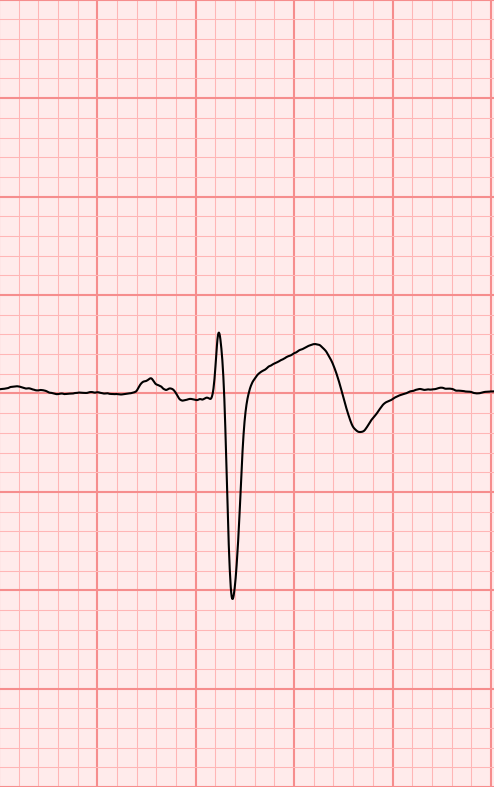
\includegraphics[width=\linewidth]{graphics/nvis_0446_v4_2_mi_st.png}
      \caption{Visualisation-absent: unannotated ECG.}
    \end{subfigure}
\hfill
    \begin{subfigure}[t]{0.24\textwidth}
      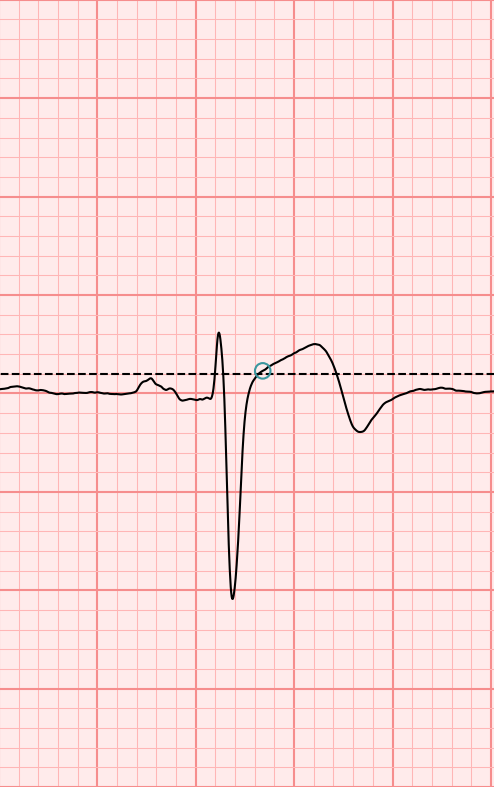
\includegraphics[width=\linewidth]{graphics/JT_0446_v4_2_MI_st.png}
      \caption{J-point Marker + Threshold Line.}
    \end{subfigure}
\hfill
    \begin{subfigure}[t]{0.24\textwidth}
      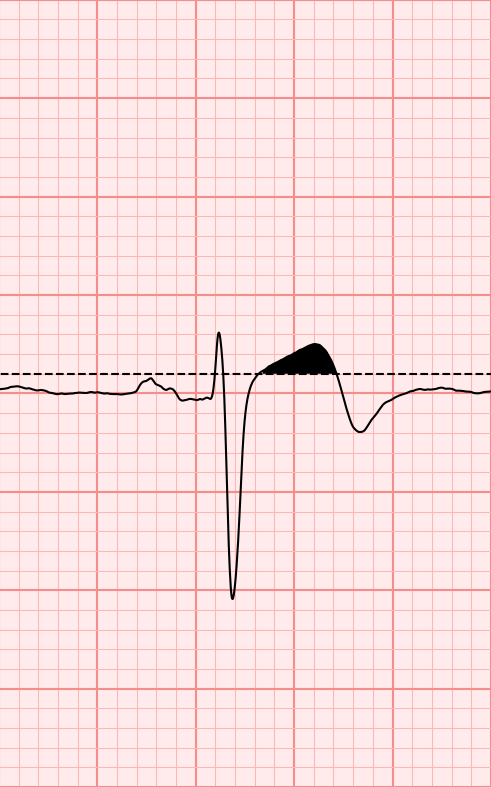
\includegraphics[width=\linewidth]{graphics/ST_0446_v4_2_MI_st.png}
      \caption{Shading + Threshold Line.}
    \end{subfigure}
\hfill
    \begin{subfigure}[t]{0.24\textwidth}
      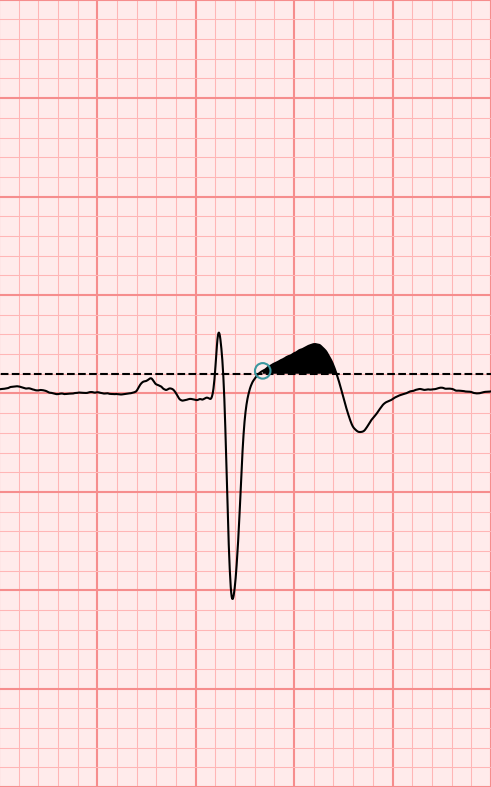
\includegraphics[width=\linewidth]{graphics/STJ_0446_v4_2_MI_st.png}
      \caption{Shading + Threshold Line + J-point Marker.}
    \end{subfigure}
  \caption{Stimuli Examples: examples of the stimuli used in the experiment in visualisation-absent and the three visualisation-present conditions. This ECG signal is taken from the V4 chest lead and has an elevated ST-segment.}
  \label{fig:vis-examples}
\end{figure}%

\subsection{Part I: Clinical Validation of
Visualisations}\label{part-i-clinical-validation-of-visualisations}

Building upon our RRI and stakeholder engagement work conducted
throughout the ECG-X project\footnote{www.ecgx.co.uk}, we conducted a
clinical validation study focused on a qualitative evaluation of the
usefulness and correctness of our visualisation designs by clinical
experts. Participants across four specialties (Anaesthesia, Critical
Care, Emergency Medicine, and Cardiology) were convenience
sampled\textasciitilde{}\cite{mason_qualitative_2018} as part of their
ongoing stakeholder engagement in the project. We aimed to recruit at
least five clinicians, a common threshold for formative medical device
and software evaluation\textasciitilde{}\citep{FDA2016HumanFactors}, and
our sample size followed established human-factors principles where
small expert samples are appropriate for formative, low risk
evaluations\textasciitilde{}\citep{IEC}. All clinicians were based in
the UK at the time of evaluation. These specialties were selected after
a series of RRI workshops, which identified these groups as regularly
interpreting ECGs. Based on the Ethics Decision Tool at the University
of Manchester and the NHS Health Research Authority Ethics
Toolkit\textasciitilde{}\cite{nhs_ethics}, the study was exempt from
ethical review as we solely consulted with professionals (i) strictly
within their professional remit, and (ii) did not collect any personally
identifiable information apart from those on the exempt list,
i.e.~names, professional roles, signed consent, and audio recordings.

The evaluations were undertaken between November 2025 and January 2026
via the video conferencing software Microsoft
Teams\textasciitilde{}\cite{ms-teams} (video function disabled).
Participants were included on the basis that they are currently employed
clinicians with ``experiential
relevance'\,`\textasciitilde{}\cite[p. 124]{rudestam_surviving_2015} in
terms of ECG usage and clinical knowledge. As we aimed to generate data
that establishes a representational account of participants'
professional roles, we refrain from including the names of clinicians.
All participants received a Participant Information Sheet (PIS) prior to
the interview and provided informed consent. Participants were further
given the option of withdrawing data up to 14\textasciitilde days after
the date of participation, and received a shopping voucher worth Fifteen
Pounds Sterling (GBP or £) as a token of appreciation for their time
investment.

The evaluations followed a semi-structured
guide\textasciitilde{}\cite{lindlof_qualitative_2017} based on
generative questions\textasciitilde{}\cite{rubin_qualitative_2005} to
encourage extensive replies in an open format. The guide was developed
during RRI workshops and is grounded in practice-based approaches of
Human-Computer Interaction (HCI) to enable investigation of
participants' lived experiences with
technologies\textasciitilde{}\cite{kuutti_turn_2014}. The guide
introduced participants to our visualisations, explained how they were
designed, and detailed that they are explainable based on clinical
rules. We then asked about their clinical correctness, usefulness, and
clinicians' preferences, followed by considerations of how they would
use them in their clinical practice.

All materials, such as the Ethics Outcomes Letters, validation study
guide, and transcripts are openly accessible and were deposited on
Figshare with consent from
participants\footnote{\url{https://doi.org/10.48420/31042243}}.

\subsection{Part II: Online Experiment with Lay
Participants}\label{part-ii-online-experiment-with-lay-participants}

Our goal was to design visualisations based on clinical rules to enable
intuitive visual identification of ST-elevation -- as commonly prevalent
in STEMI -- on ECGs. To recapitulate, that is an elevation at the
J-point of at least 0.1\textasciitilde mV in any two contiguous leads
except V2 and V3. In leads V2 and V3, this elevation must be at least
0.2\textasciitilde mV in males aged 40\textasciitilde years or older, at
least 0.25\textasciitilde mV in males aged under
40\textasciitilde years, and at least 0.15\textasciitilde mV in females.
Motivated by previous work\textasciitilde{}\citep{alahmadi_2023}, we
conducted rounds of RRI workshops with lay people, clinicians regularly
interpreting ECGs, and HCI experts to draft the following research
pathway.

Since we specifically recruited lay participants who were unfamiliar
with ECGs, simply asking participants to spot a STEMI on an ECG, whether
with or without the added visualisation, would be a task with a high
intrinsic cognitive load. Instead, we segmented this task into smaller,
more easily achievable steps. Notably, we:

\begin{enumerate}
\def\labelenumi{\arabic{enumi}.}
\item
  Solely focused on ST-elevation without introducing the concept of STEMI.
\item
  Only used leads where the 0.1~mV rule applies.
\item
  Only showed single-heartbeat single-lead images.
\item
  Removed the necessity to understand the contiguity rule and examine
  multiple leads.
\end{enumerate}

\%

Participants were trained exclusively on these principles, and were not
introduced to concepts or rules unnecessary for the completion of the
classification task. The task that participants performed can
essentially be broken down into a pair of subtasks: 1) locate the
J-point, and 2) check for the ST-elevation,
\emph{in purely descriptive terms based on the ECG images shown}.

\subsubsection{Crowdsourcing}\label{crowdsourcing}

There is precedent for work investigating ECG interpretation to feature
lay participants\textasciitilde{}\citep{alahmadi_2020}, and for
crowdsourcing to be used in health
research\textasciitilde{}\citep{crequit_2018}. These concepts have
intersected in the context of crowdsourced data labelling or
annotation\textasciitilde{}\citep{zhu_2014, bahrami_2021, bahrami_2024}.
The work presented here takes influence from psychophysics and
visualisation design studies that extensively employ crowdsourcing.
Crowdsourcing affords the rapid collection of large amounts of data, and
is considerably less expensive than traditional, in-person testing. Data
quality and demographics issues have caused concern in past
research\textasciitilde{}\citep{chmielewski_2020, peer_2021}, so here we
follow published guidelines\textasciitilde{}\citep{peer_2021} to ensure
the collection of high-quality data. The Prolific
platform\textasciitilde{}\citep{prolific} is used, along with strict
pre-screening criteria; participants were required to have previously
successfully completed at least 100 Prolific studies, and were required
to have been accepted on at least 95\% of their previous submissions.

\subsubsection{Open Research}\label{open-research}

This project was conducted according to the principles of open and
reproducible research\textasciitilde{}\citep{ayris_2018}. Hypotheses and
analysis plans were pre-registered with the Open Science Framework
(OSF)\footnote{https://osf.io/v6tjp}. All data and analysis code are
maintained in a GitHub
repository\footnote{\url{https://github.com/ECG-X/increasing_the_accuracy_of_ST-segment_elevation}},
which also contains instructions for building a Docker container to
reproduce the computational environment in which the paper was written.
This facilitates full replication of figures, analyses, and the paper
itself. The algorithm to create ECG images with visualisations is also
accessible (see Section\textasciitilde{}\ref{sec-vis-alg-dev}).

\subsubsection{Modelling}\label{modelling}

Our primary outcome measure -- participants' performance on the
ST-elevation classification task -- is binary. We hence built
Generalised Linear Mixed Models (GLMMs) of the binomial family to
analyse our data. As opposed to manually specifying random effects for
models, the \texttt{buildmer} package (version
2.12\textasciitilde{}\citep{voeten_2025}) was used in R (version
4.5.1\textasciitilde{}\citep{rcore}) to automate model syntax selection
using stepwise regression. On provision of a maximal model,
\texttt{buildmer} identifies the most complex model that successfully
converges. The \texttt{lme4} package (version
1.1-37\textasciitilde{}\citep{bates_2015}) supplies the \texttt{glmer()}
function to \texttt{buildmer} that constructs the GLMM.

\subsubsection{Stimuli}\label{stimuli}

Our stimuli were designed based on the visualisation pipeline outlined
in Section\textasciitilde{}\ref{sec-vis-alg-dev} and the core principles
of our experiment described in
Section\textasciitilde{}\ref{sec-method-online-exp}. The stimuli used in
the experiment consisted of static ECG tracings representing single
heartbeats from any of the included leads (I, II, III, aVR, aVL, aVF,
V1, V4, V5, and V6), displayed either with or without visualisations
(see Figure\textasciitilde{}\ref{fig:vis-examples}). ECG segments were
sampled to illustrate the presence or absence of ST-elevation.

Several assumptions underlie the construction of our stimuli for
experimental purposes. First, stimuli assume sufficient signal quality
for visually identifiable ECG landmarks, including baseline, J-point,
and ST-segment, such that participants can reasonably perform the
classification tasks. This was ensured by manually curating and
verifying every stimulus included in the experiment. The stimuli
\textit{without} and \textit{with} ST-elevation were selected only from
the \textit{healthy control} and \textit{myocardial infarction} groups,
respectively. Second, by presenting single-lead, single-heartbeat
images, the stimuli deliberately abstract away temporal context,
beat-to-beat variability, and multi-lead information, allowing the
experimental set-up to focus specifically on perceptual interpretation
of ST-segment elevation rather than clinical diagnosis. Third, stimuli
assume that static representations are an appropriate proxy for
assessing visual interpretability by lay people, despite ECG
interpretation in practice using longer durations and multi-lead review.
Finally, visual parameters such as scaling, grid layout, and threshold
indicators, as well as image size, were held constant across conditions
to ensure that any observed differences in performance could be
attributed to the presence or absence of visual cues rather than
differences in stimulus presentation.

These assumptions reflect the controlled nature of the experiment to
test the usefulness of visualisation -- to facilitate the interpretation
of ST-segment elevation -- and to support systematic comparison of our
conditions, rather than to replicate the complexity of real-world ECG
interpretation.

\subsubsection{Procedure}\label{procedure}

The experiments were built using
PsychoPy\textasciitilde{}\citep{peirce_2019} and hosted
on\textasciitilde{}\url{Pavlovia.org}. Participation was permitted using
laptop or desktop computers only. A flowchart depicting the experimental
procedure is presented in
Figure\textasciitilde{}\ref{fig:exp-flowchart}. Participants were first
shown the PIS and were asked to provide consent via key presses in
response to consent statements. They provided their age in a free text
box, followed by their gender identity. Participants were then taken to
a 4-minute training module. This consisted of a series of slides
outlining the general form of ECG tracings, the rules that define
ST-elevation within the experimental context (see
Section\textasciitilde{}\ref{sec-stemi} and
Section\textasciitilde{}\ref{sec-method-online-exp}), and an overview of
the particular visualisation condition that they were assigned to.
Between visualisation conditions, the training modules differed only in
terms of their final slide instructing participants how to use the
particular visualisation. The training slides are included in the
supplemental material associated with this paper. Following the training
module, participants were given four practice trials. These were
identical to the experimental trials, but provided feedback to
participants that informed them \emph{why} they were correct or
incorrect. All four practice trials featured the visualisation, with two
displaying ST-elevation present and two displaying ST-elevation absent.

\begin{figure}[H]

{\centering \pandocbounded{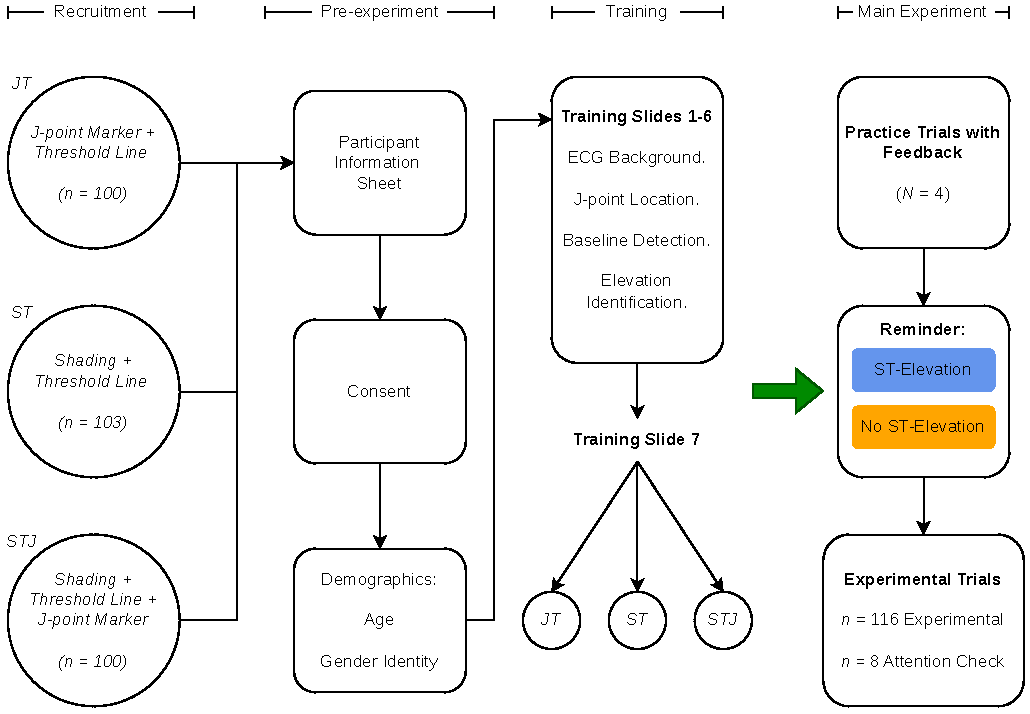
\includegraphics[keepaspectratio]{graphics/ECG_exp_flowchart.pdf}}

}

\caption{Experimental Flowchart: Flowchart depicting the stages of the
experimental procedure.}

\end{figure}%

Prior to beginning the experimental trials, participants were reminded
to press the
\texttt{ST-Elevation\textquotesingle{}\textquotesingle{}\ button\ if\ they\ believed\ the\ ECG\ showed\ ST-elevation,\ and\ to\ press\ the}No
ST-Elevation'\,' button if they did not believe the ECG showed
ST-elevation. They were warned that the positions of the buttons would
change throughout the experiment. Participants then worked through a
series of 124 trials. Each trial was preceded by text that either read
\texttt{Please\ look\ at\ the\ following\ ECG\ and\ decide\ if\ ST-elevation\ is\ present.\textquotesingle{}\textquotesingle{}\ (\$\{n\ =\ 116\}\$,\ black\ text,\ experimental\ trials)\ or}Please
IGNORE the following ECG and click on the centre of the
visualisation.'\,' (\({n = 8}\), red text, attention check trials).
There was no time limit per trial. An example of an experimental trial
can be seen in Figure\textasciitilde{}\ref{fig-example-trial}.
Participants who successfully completed the experiment were paid pro
rata through Prolific at a rate of £6 per hour.

\begin{figure}

\centering{

\pandocbounded{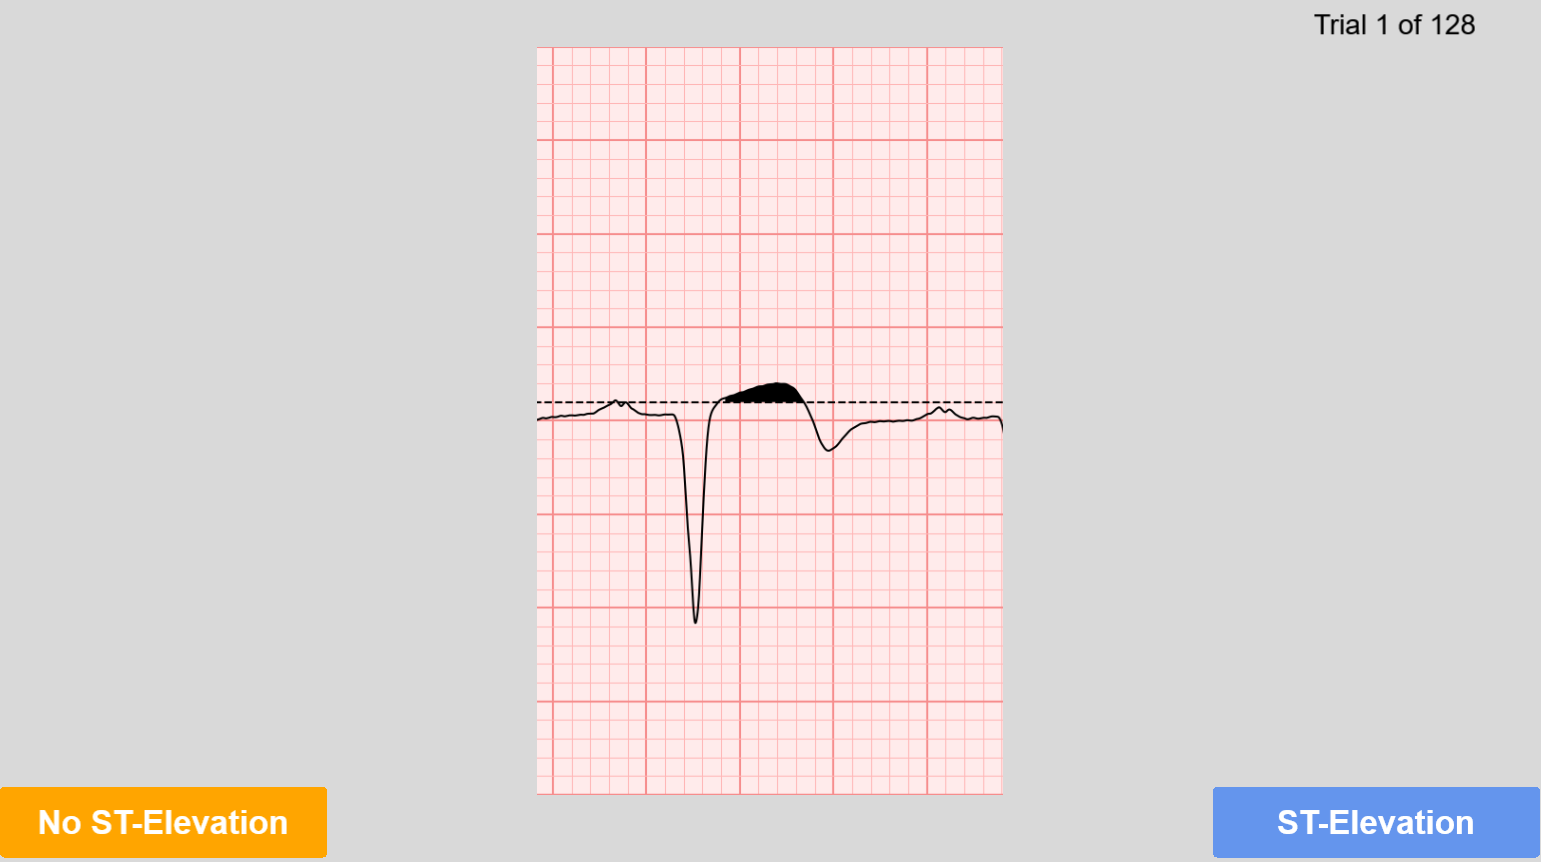
\includegraphics[keepaspectratio]{graphics/example_trial.png}}

}

\caption{\label{fig-example-trial}Example Experimental Trial: example
trial in the extit\{Shading\} + extit\{Threshold Line\} condition. This
ECG visualisation does show ST-elevation.}

\end{figure}%

All participants were recruited with the Prolific
platform\textasciitilde{}\citep{prolific}. We sought to recruit
\({n = 100}\) participants for each of the three between-participants
experiments. English fluency, normal or corrected-to-normal vision, and
having not taken part in any of the RRI workshops described in
Section\textasciitilde{}\ref{sec-method-online-exp} were required for
participation. Participants were also instructed not to take part if
they had prior medical knowledge or experience interpreting ECGs.

\subsubsection{Experimental Design}\label{experimental-design}

We employed a mixed design. Within participants, all saw the same 58 ECG
tracings without visualisations (29 with ST-elevation, 29 without). The
between-participants factor was the type of ECG visualisation utilised.
Each group saw the same 58 ECG tracings with the different
visualisations shown in Figure\textasciitilde{}\ref{fig:vis-examples}.
Participants saw 116 experimental and 8 attention check items in a fully
randomised order. Dependent variables were participant responses to ECG
stimuli and the speed with which they provided their responses. All
experimental code, materials, and instructions are hosted on GitLab as
three separate
experiments\footnote{https://gitlab.pavlovia.org/Strain/ecg_x_jt}\fnsep\footnote{https://gitlab.pavlovia.org/Strain/ecg_x_st}\fnsep\footnote{https://gitlab.pavlovia.org/Strain/ecg_x_stj}.

\section{Results}\label{results}

\subsection{Part I: Clinical Validation of
Visualisations}\label{valid-results}

\subsubsection{Preference for Distinct Visual
Cues}\label{preference-for-distinct-visual-cues}

\subsubsection{Trust in Guideline-Based
Visuals}\label{trust-in-guideline-based-visuals}

\subsubsection{Role in Contemporary Computerised Interpretation of
ECG}\label{role-in-contemporary-computerised-interpretation-of-ecg}

\subsubsection{Educational Value}\label{educational-value}

\subsubsection{Universal Application and Pre-Hospital
Utility}\label{universal-application-and-pre-hospital-utility}

\subsection{Part II: Online Experiment with Lay
Participants}\label{online-results}

\subsection{Additional Analyses}\label{additional-analyses}

\section{Discussion}\label{discussion}

\subsection{Part I: Clinical Validation of
Visualisations}\label{valid-disc}

\subsubsection{}\label{section}

\subsubsection{}\label{section-1}

\subsubsection{}\label{section-2}

\subsection{Part II: Online Experiment with Lay
Participants}\label{online-disc}

\subsubsection{Visualisation Improves
Performance}\label{visualisation-improves-performance}

\subsubsection{Visualisation Type and Mechanism of
Action}\label{visualisation-type-and-mechanism-of-action}

\section{Conclusion}\label{conclusion}

\section*{Acknowledgements}\label{acknowledgements}
\addcontentsline{toc}{section}{Acknowledgements}

We want to thank all clinicians and critical friends of the project for
their continued input as part of our Responsible Research and Innovation
stakeholder engagement. This work was funded by the Engineering and
Physical Sciences Research Council (EPSRC) under grant number
EP/X02945X/1.


\renewcommand\refname{References}
\bibliography{bibliography.bib}



\end{document}
